\documentclass[../book.tex]{subfiles}
\graphicspath{{\subfix{../images/}}}

\begin{document}
\chapter{Quadratic Functions}
\begin{introduction}[Contents]
\item Quadratics in Vertex Form
\item Quadratics in Factored Form
\item Review: Distribution and F.O.I.L.
\item Special Quadratics
\item Factoring Standard-Form Quadratics
\item Hidden Quadratics
\item Completing the Square
\item The Quadratic Formula
\item Summary of Quadratics
\end{introduction}
\noindent Quadratic Polynomials, commonly referred to as \textit{quadratics}, are polynomials of the second-degree with real coefficients.  In \hyperlink{chapter.4}{Chapter 4}, we covered linear functions in slope-intercept form, point-slope form, and standard form.  We also found a way to start at each form and arrive at another.  Our goal is to do the same for quadratics.

Like quadratics, we have a standard form.  For $a,b,c\in\mathbb{R}$ and $a\neq 0$, the standard form of a quadratic is $$f(x)=ax^2+bx+c.$$  The solutions to the quadratic equation are known as \textit{roots} or \textit{zeroes}.  The $ax^2$ term is known as the quadratic term, the $bx$ term is the linear term, and $c$ is the constant term.
\begin{wrapfigure}{r}{4cm}
    \begin{tikzpicture}[xscale=0.5,yscale=0.5]
      \draw[<->] (-3,0) -- (3,0) node[right] {$x$};
      \draw[<->] (0,-3) -- (0,3) node[above] {$y(x)$};
      \draw[scale=0.5,domain=-3:3,smooth,variable=\x,blue] plot ({\x},{\x*\x});
    \end{tikzpicture}
\end{wrapfigure}
The parent function in this chapter is $f(x)=x^2$ with domain $\mathbb{R}$.  Most of us, from Algebra I, know that the graph is a "U"-shape.  The graph of $f(x)=x^2$ is shown to the right.  We note the vertex is at $(0,0)$ and the only zero is at $(0,0)$.  The next challenge is to determine how to graph the same function if there is a linear and constant term.  We'll have to resort to the other two forms.

This chapter will detail the processes for solving quadratics of all different types as well as an easy-to-follow method for graphing quadratics.
\section{Quadratics in Vertex Form}
\noindent The first type of quadratics that we will deal with are quadratics in vertex form.  These quadratics highlight the vertex of the polynomial and the measure of compression.  The form of a quadratic in vertex form is $$y(x)=a(x-h)^2+k.$$  In this case, $a$ is the measure of compression while $(h,k)$ is the vertex of the polynomial.  Note that this $a$ is the same $a$ that was in the standard form in the introduction!  This means that the same value of $a$ in the standard form also represents the measure of compression.

If a quadratic is in vertex form, it can be solved with square roots.  To solve this, we follow a very simple process.  First, rearrange the equation to isolate the square.  Then, take the square root of both sides and note the two resultant solutions.  Solve each resultant equation separately for $x$.  Let's try a few examples of this.
\begin{example}
Solve $(x+1)^2-6=0$.
\end{example}
\begin{solution}
Isolating the squared quantity, we get $(x+1)^2=6$.  Take the square root: $x+1=\pm\sqrt{6}$, meaning that $x_1=-1-\sqrt{6}$ and $x_2=-1+\sqrt{6}$.  $\Box$
\end{solution}
\begin{example}
Solve $2(x-3)^2-9=9$.
\end{example}
\begin{solution}
Isolate the squared quantity: $(x-3)^2=9$.  Take the square root: $(x-3)=\pm 3$.  Solve for $x$: $x_1=0$ and $x_2=6$.$\Box$
\end{solution}
\begin{example}
Solve $3(x-1)^2=0$.
\end{example}
\begin{solution}
Isolate the squared quantity: $(x-1)^2=0$.  Take the square root: $(x-1)=0$.  Solve for $x$: $x_{1,2}=1$.$\Box$
\end{solution}
\begin{example}
Solve $2(x+2)^2+12=6$.
\end{example}
\begin{solution}
Isolate the square quantity: $(x+2)^2=-3$.  Take the square root: $(x+2)=\pm i\sqrt{3}$.  Solve for $x$: $x_1=-2-i\sqrt{3}$ and $x_2=-2+i\sqrt{3}$.  $\Box$
\end{solution}
Let's review transformations for functions in vertex form.  While this was covered generally for functions in \hyperlink{section.2.4}{Section 2.4}, we will specifically cover quadratics in vertex from for this.

The vertex form is a shifted form of the parent function $f_0(x)=x^2$.  To reach the general form $f(x)=a(x-h)^2+k$, $f_0(x)$ is shifted to the right $h$ units, up $k$ units, and is horizontally stretched by a factor of $|a|$.  If $a<0$ then $f(x)$ is inverted.  Let's attempt an example.
\begin{wrapfigure}{r}{4cm}
    \begin{tikzpicture}[xscale=0.25,yscale=0.25]
      \draw[<->] (-10,0) -- (10,0) node[right] {$x$};
      \draw[<->] (0,-10) -- (0,10) node[above] {$y(x)$};
      \draw[scale=1,domain=-2.7:4.7,smooth,variable=\x,blue] plot ({\x},{\x*\x-2*\x-3}) node[right] {$f(x)$};
    \end{tikzpicture}
\end{wrapfigure}
\begin{example}
Sketch $f(x)=(x-1)^2-4$.
\end{example}
\begin{solution}
The vertex of the quadratic is at $(1,-4)$.  Since $a=1>0$, it is upright.  We get the $y$-intercept to be $(-1)^2-4=-3$.  Solving $f(x)=0$, we get $(-1,0)$ and $(3,0)$ for the $x$-intercepts.  (Be sure to check this!)  Using the basic shape of a quadratic, we get the graph to the right.  $\Box$
\end{solution}
Let's discuss domain and range with quadratics.  Because quadratics are polynomials, quadratics are bounded on $\mathbb{R}$.  Depending on the orientation of the quadratic, the vertex will either indicate the minimum or maximum for the range.  If $a>0$ (oriented upward), then the vertex represents the minimum.  If $a<0$ (oriented downward), the vertex represents the maximum.  Let's look at an example where $f(x)$ is given a domain restriction.
\begin{example}
Let $f(x)=2(x-3)^2+1$ on $-1\leq x\leq 5$.  Find the range of $f$.
\end{example}
\begin{solution}
The important points in this case are the end points and the vertex.  Why?  Because a quadratic only ever changes direction once: at the vertex.  Thus, there will be no other critical point that gives the maximum or minimum other than these points.  The vertex is at $(3,-1)$.  We get that $f(-1)=2(-4)^2+1=33$ and $f(5)=2(2)^2+1=9$.  Since the minimum is at $(3,-1)$ and the maximum is at $(-1,33)$, we get the range to be $y\in[-1,33]$.  $\Box$
\end{solution}
\begin{remark}
  The idea of looking for a minimum and maximum by checking all "critical points" and the endpoints is known as the \textit{closed interval test}.
\end{remark}
For the last example of this section, our goal is to determine a quadratic equation from the graph.  Using the graph, we need to identify the vertex and one point on the graph.  The easiest point to use is either the $y$-intercept or an $x$-intercept.  Consider the example below.
\begin{wrapfigure}{r}{4cm}
    \begin{tikzpicture}[xscale=0.175,yscale=0.175]
      \draw[<->] (-15,0) -- (15,0) node[right] {$x$};
      \draw[<->] (0,-15) -- (0,15) node[above] {$y(x)$};
      \draw[scale=1,domain=-2.2:5.2,smooth,variable=\x,blue] plot ({\x},{-2*\x*\x+6*\x+8}) node[above right] {$f(x)$};
      \filldraw[blue] (1.5,12.5) circle[radius=7pt] node[above right] {$\left(\frac{3}{2},\frac{25}{2}\right)$};
      \filldraw[blue] (0,8) circle[radius=7pt] node[above left] {$(0,8)$};
    \end{tikzpicture}
\end{wrapfigure}
\begin{example}
Find the function $f(x)$ determined by the graph to the right.
\end{example}
\begin{solution}
We know that the basic form of the quadratic is $f(x)=a(x-h)^2+k$.  The vertex, $(h,k)$ is $\left(\dfrac{3}{2},\dfrac{25}{2}\right)$.  Now we have $f(x)=a\left(x-\dfrac{3}{2}\right)^2+\dfrac{25}{2}$.  To find $a$, we needed another point.  Plugging in the $y$-intercept, we get $8=a\left(0-\dfrac{3}{2}\right)^2+\dfrac{25}{2}$.  Simplifying, we get $-\dfrac{9}{2}=\dfrac{9}{4}a$, meaning $a=-2$.  Since $a<0$, we know that the parabola should be inverted (which it is).  So, the final result is $f(x)=-2\left(x-\dfrac{3}{2}\right)^2+\dfrac{25}{2}$.  $\Box$
\end{solution}
This concludes our study of the vertex form.  We will return to the vertex form in \hyperlink{section.5.7}{Section 5.7} when we learn to convert from standard from to vertex form.  
\section{Quadratics in Factored Form}
This section involves quadratics found in factored form.  These quadratics highlight the measure of compression and the $x$-intercepts.  The form of a quadratic in factored form is $$y(x)=a(x-\lambda_1)(x-\lambda_2)$$ where $\lambda_1$ and $\lambda_2$ are the $x$-intercepts of the polynomial.  Again, $a$ refers to the measure of compression, just as in the vertex and standard forms.  

Recall the zero product property.
\begin{theorem}{The Zero-Product Property}{zpp}
Given two expressions $a$ and $b$, if $ab=0$, then one of three possibilities must happen: \newline 
{\centering 1.  $a=0$ \hspace{35mm} 2.  $b=0$ \hspace{35mm} 3.  $a=b=0$}
\end{theorem}
If a quadratic is in the factored form, we will solve it using the zero product property.  Let's look at some examples to understand this.
\begin{example}
Solve $2x(x-1)=0$.
\end{example}
\begin{solution}
Splitting this into two factors and using the zero product property, we get $2x=0$ and $x-1=0$.  Solve both for $x$: $x_1=0$ and $x_2=1$.  $\Box$
\end{solution}
\begin{example}
Solve $(x+3)(x-4)=0$.
\end{example}
\begin{solution}
Splitting and using the zero product property gives $x+3=0$ and $x-4=0$.  Solving for $x$ gives $x_1=-3$ and $x_2=4$.  $\Box$
\end{solution}
\begin{example}
Solve $(2x-3)(3x+1)=0$.
\end{example}
\begin{solution}
Split the equations: $2x-3=0$ and $3x+1=0$.  Solving for $x$ gives $x_1=-\dfrac{1}{3}$ and $x_2=\dfrac{3}{2}$.  Note that we switched around the equations to keep our answers in ascending order.  $\Box$
\end{solution}
\begin{example}
Solve $(4x-5)^2=0$.
\end{example}
\begin{solution}
This is the same as saying $(4x-5)(4x-5)=0$.  Splitting, we get $4x-5=0$, meaning $x_{1,2}=\dfrac{5}{4}$.$\Box$
\end{solution}
Now let's discuss the idea of graphing quadratics in factored form.  When in this form, we are given the $x$-intercepts and want to find a vertex.  Recall that a quadratic is symmetric about a central vertical line containing the vertex, called the \textit{axis of symmetry}.  Since this is true, we can find the axis of symmetry by taking the average of the roots.  Why?  The roots are at the same $y$-coordinate, meaning that the average will represent the axis of symmetry at $y=0$.  If you graph various functions, you will see that this is true for all quadratic functions.  To find the $y$-coordinate of the vertex, simply plug in the $x$-coordinate into $y(x)$.  

Let's try to graph a few examples.
\begin{example}
Graph $f(x)=(x+1)(x-7)$.
\end{example}
\begin{solution}
The $x$-intercepts given here are at $x_1=-1$ and $x_2=7$.  To find the vertex, we take the average of the $x$-intercepts, which means $h=\dfrac{-1+7}{2}=3$.  To find $k$, plug this into $f(x)$.  So, $f(3)=(3+1)(3-7)=-16$.  Thus, the vertex is at $(3,-16)$.  The graph is shown on the top of the next page.  $\Box$
\end{solution}
\begin{example}
Graph $g(x)=-2(x-2)(x-8)$.
\end{example}
\begin{solution}
The $x$-intercepts given here are at $x_1=2$ and $x_2=8$.  To find the vertex, we take the average, which is $\dfrac{2+8}{2}=5$.  Finding the $y$-coordinate of the vertex, we get $g(5)=-2(5-2)(5-8)=18$; thus, the vertex is $(5,18)$.  We plot the parabola given these three points, and is shown on the top of the next page.  $\Box$  
\end{solution}
\begin{figure}[!ht]
\centering
    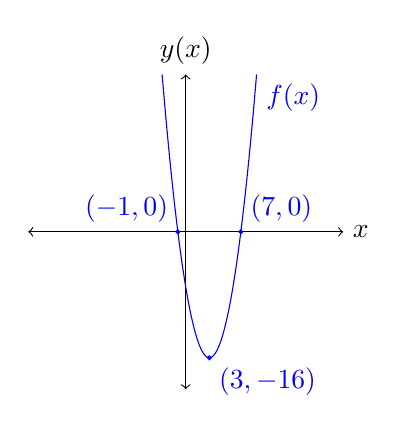
\begin{tikzpicture}[xscale=0.10,yscale=0.10]
      \draw[<->] (-20,0) -- (20,0) node[right] {$x$};
      \draw[<->] (0,-20) -- (0,20) node[above] {$y(x)$};
      \draw[scale=1,domain=-3:9,smooth,variable=\x,blue] plot ({\x},{\x*\x-6*\x-7}) node[below right] {$f(x)$};
      \filldraw[blue] (3,-16) circle[radius=7pt] node[below right] {$(3,-16)$};
      \filldraw[blue] (7,0) circle[radius=7pt] node[above right] {$(7,0)$};
      \filldraw[blue] (-1,0) circle[radius=7pt] node[above left] {$(-1,0)$};
    \end{tikzpicture}
    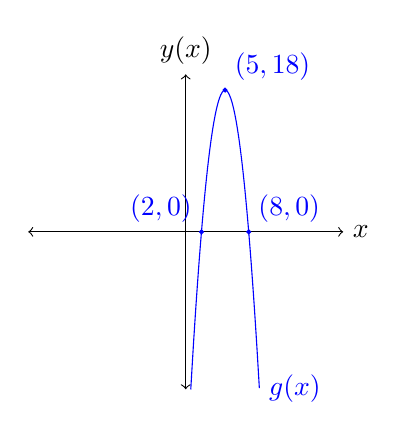
\begin{tikzpicture}[xscale=0.10,yscale=0.10]
      \draw[<->] (-20,0) -- (20,0) node[right] {$x$};
      \draw[<->] (0,-20) -- (0,20) node[above] {$y(x)$};
      \draw[scale=1,domain=0.64:9.35,smooth,variable=\x,blue] plot ({\x},{-2*\x*\x+20*\x-32}) node[right] {$g(x)$};
      \filldraw[blue] (5,18) circle[radius=7pt] node[above right] {$(5,18)$};
      \filldraw[blue] (8,0) circle[radius=7pt] node[above right] {$(8,0)$};
      \filldraw[blue] (2,0) circle[radius=7pt] node[above left] {$(2,0)$};
    \end{tikzpicture}
\end{figure}
This was a pretty simple section.  One last skill you should ensure you know is how to find the equation given a graph.  All you need to do is find the $x$-intercepts, then use another point to determine the compression factor (usually the $y$-intercept or the vertex works very well).  The rest of the chapter covers the methods to convert between forms; we begin with converting from factored form to standard form.
\section{Review: Distribution and F.O.I.L.}
\noindent This section solely covers material that was introduced in Algebra I.  Students should be very familiar with the method reviewed in this chapter and should be comfortable applying it in various situations.  Consider an expression in the form $$(a+b)(c+d)$$ where $a,b,c,d\in\mathbb{R}$.  There are two ways to derive this formula - algebraically and geometrically - and we will derive it both ways.  The first method is using the distributive property (like \hyperlink{chapter.3}{Chapter 3}).  If we distribute the $(c+d)$ term to the left side, we get $$(a+b)(c+d)=a(c+d)+b(c+d).$$  

\begin{wrapfigure}{r}{7cm}
    \centering
\begin{tikzpicture}
    \draw[black] (0,0) rectangle ++(5,5);
    \draw[black] (0,0) rectangle ++(4,1);
    \draw[black] (0,0) rectangle ++(5,1);
    \draw[black] (0,0) rectangle ++(4,5);
    \draw[|<->|] (0,5.5) -- node[fill=white,sloped] {$a$} (4,5.5);
    \draw[|<->|] (4,5.5) -- node[fill=white,sloped] {$b$} (5,5.5);
    \draw[|<->|] (-0.5,1) -- node[fill=white,sloped,rotate=270] {$c$} (-0.5,5);
    \draw[|<->|] (-0.5,0) -- node[fill=white,sloped,rotate=270] {$d$} (-0.5,1);
    \node at (2,0.5) {$ad$};
    \node at (4.5,0.5) {$bd$};
    \node at (2,3) {$ac$};
    \node at (4.5,3) {$bc$};
\end{tikzpicture}
\end{wrapfigure}

Then, use the distributive property to split it.  $$a(c+d)+b(c+d)=ac+ad+bc+bd.$$  That's the split form!  Now let's try the geometric method.  Consider the figure to the right where the area of each rectangle was marked inside.  If we find the area of the largest rectangle, we get the area as $(a+b)(c+d)$.  Adding up the smaller areas, we get $ac+ad+bc+bd$.  This must mean that $$(a+b)(c+d)=ac+ad+bc+bd.$$  This is what we got then first time!

\begin{remark}
Again, like most of the ideas or formulas we derive, don't memorize it.  It's not beneficial; it's much better to understand how to apply it and its derivation.
\end{remark}

This brings what we call the F.O.I.L.  method for multiplying two binomial expressions.  FOIL is an acronym that stands for "First, Outer, Inner, Last" which reminds students how to multiply the binomials.  Let's try a few examples to make sure that we understand the acronym and how it works.
\begin{example}
Expand $(x-2)(x+3)$.
\end{example}
\begin{solution}
Following FOIL, we multiply the first terms ($x\cdot x=x^2$), the outer terms ($x\cdot 3=3x$), the inner terms ($-2\cdot x=-2x$) and the last terms ($-2 \cdot 3=-6$).  Then, adding them up we get $$x^2+3x-2x-6 \implies x^2+x-6.$$ $\Box$
\end{solution}
\begin{example}
Expand $(2x+3)(1-x)$.
\end{example}
\begin{solution}
Following FOIL, we get $2x-2x^2+3-3x=-2x^2-x+3$.$\Box$
\end{solution}
\noindent This section is super short because we just wanted to cover this topic.  We now will move on to special types of quadratics and their properties.
\section{Special Quadratics}
\noindent This section will cover the properties of two special types of quadratics.  We've already seen one of them; we just haven't given it a formal name nor explored it in more detail.

The first special quadratic is the \textit{perfect square trinomial}.  Look at the definition below.
\begin{definition}{Perfect Square Trinomials}{pst}
A perfect square trinomial is defined that, for some real functions $a$ and $b$, $$(a\pm b)^2=a^2\pm 2ab+b^2.$$
\end{definition}
We've done a few examples with these in previous sections.  This is super easy to prove using FOIL, so we challenge you to try this for yourself.  Let's look at a few distribution and factoring examples.
\begin{example}
Expand $(2x-3)^2$.
\end{example}
\begin{solution}
You can either use the formula or use FOIL.  Either way, it produces the same result.  Following the formula, we get $(2x)^2-2(2)(3)+(3)^2=4x^2-12x+9$.  $\Box$
\end{solution}
\begin{example}
Factor $49x^2+28x+4$.
\end{example}
\begin{solution}
All we need to do is follow the definition in reverse.  We see that $49x^2+28x+4=(7x)^2+2(7)(2)+(2)^2=(7x+2)^2$.  $\Box$
\end{solution}
The second special quadratic is the \textit{difference of squares}.  Look at the definition below.
\begin{definition}{Difference of Squares}{dos}
The difference of squares is defined that, for some real functions $a$ and $b$, $$a^2-b^2=(a+b)(a-b).$$
\end{definition}
We haven't seen this example yet, so we will prove it.  There are two ways of proving this: algebraically and geometrically.  The algebraic method involves proving it using FOIL.  All we need to do is expand the right side of the equation.  $$(a-b)(a+b)=a^2+ab-ab-b^2=a^2-b^2.$$
The second way of proving this is geometrically.  Imagine a square with length $a$ where we cut off a slice of length $b$, as seen in the first figure.  We then attach it to the other side to produce the second figure.

\begin{figure}[!ht]
    \centering
    \begin{tikzpicture}[xscale=0.5,yscale=0.5]
      \draw (-3,-3) rectangle (3,3);
      \draw[dashdotted] (-3,-2) -- (3,-2);
      \draw[|<->|] (-3,3.75) -- node[fill=white,sloped] {$a$} (3,3.75); 
      \draw[|<->|] (-3.75,-3) -- node[fill=white,sloped] {$b$} (-3.75,-2);
    \end{tikzpicture} $\Longrightarrow$  
    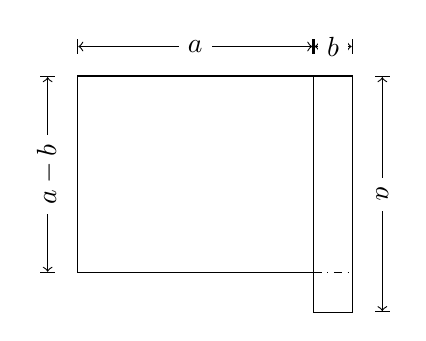
\begin{tikzpicture}[xscale=0.5,yscale=0.5]
      \draw (-3,-2) rectangle (3,3);
      \draw (3,-3) rectangle (4,3);
      \draw[|<->|] (-3,3.75) -- node[fill=white,sloped] {$a$} (3,3.75); 
      \draw[|<->|] (3,3.75) -- node[fill=white,sloped] {$b$} (4,3.75);
      \draw[|<->|] (-3.75,-2) -- node[fill=white,sloped] {$a-b$} (-3.75,3);
      \draw[|<->|] (4.75,-3) -- node[fill=white,sloped,rotate=180] {$a$} (4.75,3);
      \draw[dashdotted] (3,-2) -- (4,-2);
    \end{tikzpicture}   
\end{figure}

We then find the area of each figure.  The area of the first figure is $a^2$ as it is a square.  The area of the second square can be done in parts.  To get the formula we want, we will divide it into the entire upper rectangle and the small square on the bottom (as separated by the dashed line).  The area of this is $(a+b)(a-b)+b^2$.  These should be equal, meaning $$a^2=(a+b)(a-b)+b^2 \implies a^2-b^2=(a+b)(a-b).$$
As we can see, this is the formula in the definition box, so we know we have it correct.

Now, let's try a few examples of this to ensure we understand how use it.
\begin{example}
Distribute $(2x-3)(2x+3)$.
\end{example}
\begin{solution}
Following the formula, we know that the expanded form is $(2x)^2-(3)^2=4x^2-9$.  $\Box$
\end{solution}
\begin{example}
Factor $63x^2-175$.
\end{example}
\begin{solution}
Factor out the common factor of $7$.  This gives $7(9x^2-25)$, which factors to $7(3x-5)(3x+5)$.$\Box$ 
\end{solution} 
This is all we needed to cover regarding these.  We simply wanted to ensure you were aware of these special forms so you can use them to your advantage.  Now, let's discuss one of the toughest sections in this chapter: factoring.
\section{Factoring Standard-Form Quadratics}
\noindent This may be one of the tougher sections of this chapter and is definitely the most difficult to teach.  There are many ways to factor quadratics, where some are more efficient than others.  In this process, we will disregard any factoring method you may know and discuss the methods we find to be most effective.  

There are three methods in this section, where each method builds on another.  It is very important you understand the previous methods as you move on to the more difficult, as they become more difficult to understand and more intuitive.  We outline each method in its own subsection; it is imperative that you attempt each problem on your own before reviewing the solution.
\subsection{Splitting the Middle Term}
\noindent This is the most common factoring technique that used to be taught in schools.  Schools now are using a visual factoring method that we find to be a waste of time and space.  Splitting the middle term offers the best value for the time spent learning and practicing, which makes it a good investment.

The goal of splitting the middle term (and every other method) is to find two numbers that multiply to the constant term and add to the linear term.  The derivation for this is explained in the \hyperlink{section.5.5.2}{next} subsection.  Once we do this, we "split" the middle term into these two factors and the \textit{factor by grouping}.  Let's try this.
\begin{example}
Factor $x^2+6x+8=0$.
\end{example}
\begin{solution}
We need two numbers that multiply to $8$ and add to $6$.  Let's consider the factors of $8$: $1$, $2$, $4$, and $8$.  Right away we see that $2+4=6$.  To split the middle term, we simply rewrite the function as $x^2+\left(2x+4x\right)+8$.  Now, we factor by grouping.  To do this, we simply find the greatest common factor of the first two terms and of the last two terms.  This looks like $$x^2+2x+4x+8=x(x+2)+4(x+2).$$  We then factor the $(x+2)$ from both terms to get $$x(x+2)+4(x+2)=(x+4)(x+2).$$ $\Box$
\end{solution}
Let's add some negatives to the problem to see how it changes the way we look at it.
\begin{example}
Factor $x^2-3x-10=0$.
\end{example}
\begin{solution}
We need two numbers that multiply to $-10$ and add to $-3$.  We know that these two numbers must have opposite signs and that the larger number must be negative.  The factors of $10$ are $1$, $2$, $5$, and $10$, and the pair that works is $-5$ and $2$.  Splitting the middle term, we get $$x^2-5x+2x-10=0.$$  Factoring by grouping gives $$x(x-5)+2(x-5) \implies (x+2)(x-5)=0.$$ $\Box$
\end{solution}
What happens when $a\neq 1$?  The problem doesn't become so easy.  We do have a method for this; however, that makes it seem as easy as this first type of problem.  We will use the method of bringing the leading coefficient to the back and factor as normal.
\begin{example}
Factor $2x^2+5x-3=0$.
\end{example}
\begin{solution}
If we bring the leading coefficient ($2$) to the back, we get the new equation $x^2+5x-6=0$.  This is something we know how to factor!  We look for two numbers that multiply to $-6$ and add to $5$.  Considering the factors of $6$, we have $1$, $2$, $3$, and $6$.  The factor pair that adds to $5$ when the pair has opposite signs is $6$ and $-1$ (Do not fall for the $2$ \& $3$ pair trap!)  Splitting the middle term, we get $$x^2+6x-x-6=0 \implies x(x+6)-(x+6)=0 \implies (x+6)(x-1)=0.$$  

But we're not done!  Note that you don't get the original equation if you FOIL our solution.  Essentially, we multiplied the constant term by 2 in order to factor it; thus, we need to divide the constants by $2$.  This gives $$\left(x+3\right)\left(x-\dfrac{1}{2}\right)=0.$$  Instead of writing the second term like this, we move the $2$ to the $x$ term and the root doesn't change (be sure you see why).  This gives the factors $$(x+3)(2x-1)=0.$$ $\Box$
\end{solution}
The only time that this method is ineffective is when the values of $a$, $b$, and $c$ are large; there would be a lot of factors to go through.  This is best dealt with in the next section when we discuss factoring via coefficients.
\subsection{Factoring via Coefficients}
\noindent This is a tough method to learn.  It involves solving simple systems of equations by understanding a little about number theory.  This method, along with the next one, require a great deal of number sense with respect to divisibility, multiplication of (sometimes large) numbers, and factors of commonly seen numbers.

Let's try and derive the ideas we will need in this section.  Given two roots of a polynomial, $\lambda_1$ and $\lambda_2$, we know that the quadratic must be in the form $$(x+\lambda_1)(x+\lambda_2)=x^2+\left(\lambda_1+\lambda_2\right)x+\lambda_1\lambda_2.$$  That means, we know that we have a system of equations here.  If $f(x)=x^2+bx+c$ (assuming $a=1$), we know that $\lambda_1+\lambda_2=b$ and $\lambda_1\lambda_2=c$.  To factor the quadratic, we need to solve for $\lambda_1$ and $\lambda_2$.  We aren't going to find a solution in terms of $b$ and $c$; instead we will find a solution case-by-case.

Let's try a few examples to get the hang of this idea.
\begin{example}
Factor $x^2-13x+36=0$.
\end{example}
\begin{solution}
We know that $\lambda_1+\lambda_2=-13$ and $\lambda_1\lambda-2=36$.  Because $\lambda_1\lambda_2>0$, $\lambda_1$ and $\lambda_2$ have the same sign, and since $\lambda_1+\lambda_2<0$, we know that $\lambda_1$ and $\lambda_2$ are both negative.

Consider the factors of $36$.  We have $(1,36)$, $(2,18)$, $(3,12)$, $(4,9)$, and $(6,6)$.  The $(4,9)$ pair is the only pair that adds to $13$, so our factors are $(x-4)(x-9)$.  $\Box$ 
\end{solution}
\begin{example}
Find the roots of $x^2-12x-540=0$.
\end{example}
\begin{solution}
The numbers just got much bigger.  We know that $\lambda_1\lambda_2=-540$ and $\lambda_1+\lambda_2=-12$.  Since $\lambda_1\lambda_2<0$, we know that $\lambda_1$ and $\lambda_2$ have different signs.  Since $\lambda_1+\lambda_2<0$, the larger number must be negative.  Since $540$ has $12$ pairs of factors, and we don't want to go through all these factors, we will find an alternate solution.

Let's determine if $\lambda_1$ and $\lambda_2$ have any common factors.  We first note that $12$, $540$, and $0$ are all even.  If $x$ is odd, then the quadratic is odd and thus can't equal zero (be sure to check this for yourself).  This means that the roots are even.

We also note that $12$, $540$, and $0$ are divisible by three.  Using the same logic as the previous paragraph, we know that the roots must be divisible by $3$.

Using basic divisibility rules, we know that the roots must be divisible by $6$ as well.  We then define new roots, $\mu_1$ and $\mu_2$, such that $6\mu_1=\lambda_1$ and $6\mu_2=\lambda_2$.  This means that $6\mu_1+6\mu_2=-12$, so $\mu_1+\mu_2=-2$.  Also, $\left(6\mu_1\right)\left(6\mu_2\right)=-540$, so $\mu_1\mu_2=-15$.  This is much easier to solve.  We quickly see that $\mu_1=-5$ and $\mu_2=3$, meaning that $\lambda_1=-30 $ and $\lambda_2=18$.  Thus, our factors are $$x^2-12x-540=(x+18)(x-30)=0,$$ meaning that $x_1=-18$ and $x_2=30$.  $\Box$
\end{solution}
Up until now, we've only dealt with cases where $a=1$.  What if $a\neq 1$?  Can we write the same equations?  The short answer is: no.  Let's look at an example where this applies.
\begin{example}
Factor $3x^2+11x+10=0$.  
\end{example}
\begin{solution}
In this case, $a=3$.  This problem is slightly easier since $3$ is prime; it means there's only one pair that works: $3x\cdot x=3x^2$.  This means we write the factors as $(3x+\lambda_1)(x+\lambda_2)$.  FOILing this gives $$(3x+\lambda_1)(x+\lambda_2)=3x^2+(\lambda_1+3\lambda_2)x+\lambda_1\lambda_2.$$  So, we need to find values for $\lambda_1$ and $\lambda_2$ that satisfy $\lambda_1+3\lambda_2=11$ and $\lambda_1\lambda_2=10$.  The factor pairs of $10$ are $(1,10)$, $(2,5)$, $(5,2)$, and $(10,1)$.  Unlike Example 5.20, the order does matter here because of the different coefficients on $x$.  The only factor pair that works here is $(5,2)$, meaning $3x^2+11x+10=(x+5)(x+2)$.  $\Box$
\end{solution}
Now, what if $a$ isn't prime?  This means we need to introduce two new variables into the equation.
\begin{example}
Factor $9x^2+88x-20=0$.
\end{example}
\begin{solution}
In this case, $a=9$ has three factor pairs ($(1,9)$, $(3,3)$, and $(9,1)$).  So, we introduce two new variables $\mu_1$ and $\mu_2$ to represent that coefficient.  Thus, the factors are $(\mu_1x+\lambda_1)(\mu_2x+\lambda_2)$.  This expands to $$(\mu_1x+\lambda_1)(\mu_2x+\lambda_2)=(\mu_1\mu_2)x^2+\left(\mu_1\lambda_2+\mu_2\lambda_1\right)x+\lambda_1\lambda_2.$$
This gives the system of equations $\mu_1\mu_2=9$, $\mu_1\lambda_2+\mu_2\lambda_1=88$, and $\lambda_1\lambda_2=-20$.  But wait!  This is a four variable, three equation system.  This isn't possible!  There is a fourth restriction though - each variable must be an integer.

Let's consider this solution logically.  $88$ is a very big positive number.  $\lambda_1\lambda_2<0$, meaning that either $\lambda_1$ or $\lambda_2$ is negative.  We quickly deduce that $\lambda_1$ must be a (small) negative number.  We know that both $\mu_1$ and $\mu_2$ must be positive for this to work, and must have a significant size difference.  Let $\mu_1=9$ and $\mu_2=1$.  This means that $9\lambda_2+\lambda_1=88$.  The only solution that works here is $\lambda_1=-2$ and $\lambda_2=10$.  

Thus, our factors are $(9x-2)(x+10)$.  $\Box$
\end{solution}
These are the different types of coefficient factoring.  Let's move on to intuitive factoring, a more mental solution that combines the last two methods.
\subsection{Intuitive Factoring}
\noindent This section is undoubtedly the hardest to teach, the hardest to learn, the one that requires the most practice, yet the most rewarding.  Once you understand how to use it, you will be factoring at lightning speeds with amazing accuracy.  Essentially, this method is the previous one without showing as much work nor thinking as hard.

This method is more like the first method as it looks for the numbers that multiply to the constant and add to the linear term.  However, this method can be used for larger values of $a$, $b$, and $c$ without too much difficulty.

Let's try a few examples of this that cover various cases of intuitive factoring.
\begin{example}
Factor $x^2-x-12=0$.
\end{example}
\begin{solution}
We need two numbers that multiply to $-12$ and add to $-1$.  Instead of listing every factor, let's consider the solution intuitively.  The numbers we need must have opposite sign and the larger must be negative.  We also know they are close in magnitude, since their sum is near zero.  So, we look for two factors near $\sqrt{12}\approx 3.5$ (be sure you know why!).  The two factors that work here are $-4$ and $3$, so our factors are $(x-4)(x+3)$.  $\Box$
\end{solution}
\begin{example}
Factor $x^2-7x-18=0$.
\end{example}
\begin{solution}
We need two numbers that multiply to $-18$ and add to $-7$.  We know that they must be of opposite sign and should have a somewhat-large difference.  We also know that the larger number must be negative.  Since the linear term is near half the constant term, we should look for a root around $2$ and the corresponding roots (in this case $-9$).  We see that $-9$ and $2$ works, so the factors are $(x-9)(x+2)=0$.$\Box$
\end{solution}
Let's move on to a few examples where $a\neq 1$.
\begin{example}
Factor $2x^2-17x+35=0$.  
\end{example}
\begin{solution}
The number are getting slowly bigger and now there's a leading coefficient.  Since $2$ is prime, the only way to use it is $(2x+\lambda_1)(x+\lambda_2)$.  Since $35$ is positive, the numbers must have the same (negative) sign.  Again, since the difference between the coefficients of $x$ is low, and since the linear term is about half the constant term, the constants will be approximately equal.  The smaller of the two constants will usually be multiplied by the higher $x$-coefficient.  We pick $-5$ and $-7$ as the factors of $35$ and note that $(2)(-5)+(1)(-7)=-17$.  When you multiply these terms, according to FOIL, we put them in the \textbf{opposite} factor.  So, the factors become $(2x-7)(x-5)=0$.  $\Box$
\end{solution}
\begin{remark}
  This problem can also be solved by bringing $2$ to the back and factoring as usual.  We will do this in the next example.
\end{remark}
This last one was probably tough to follow.  Again, this method is not easy.  But once you understand a bit of the number theory behind it, it becomes a lot easier.

Let's try one where $a$ isn't prime.
\begin{example}
Factor $6x^2+11x-10$.
\end{example}
\begin{solution}
Since $a$ isn't prime, and there's not a good way to deal with this, we bring it to the back.  This gives $x^2+11x-60=0$.  Since the middle term is approximately a quarter of the constant term, we try the roots $15$ and $-4$.  They work!  This gives the factors $(x+15)(x-4)=0$.  We then divide the constants by $6$ to get $$(x+15)(x-4)\implies \left(x+\dfrac{5}{2}\right)\left(x-\dfrac{2}{3}\right)\implies (2x+5)(3x-2)=0.$$ $\Box$
\end{solution}
These are the essentials of intuitive factoring.  Continue to practice it as we move on to hidden quadratics, where we find secret quadratics inside of seemingly impossible functions.
\section{Hidden Quadratics}
\noindent The goal of this section is to learn to factor "hidden" quadratics.  Hidden quadratics are quadratic functions where the $x$-variable is some other function, such as an exponential, trigonometric, or other.  All we need to do is make a substitution to make the quadratic into a function we know how to factor and solve it.

Let's look at a few examples to understand how to solve it.  
\begin{example}
Solve $\left(3^x\right)^2-12\left(3^x\right)+27=0$.
\end{example}
\begin{solution}
We see that we almost have a quadratic if it weren't for the $3^x$ terms.  So, we make what's known as a \textbf{u-substitution}.  In this case, we let $u=3^x$.  Why?  This will help us to remove both $3^x$ terms and leave a quadratic!
$$\left(3^x\right)^2-12\left(3^x\right)+27=0 \implies u^2-12u+27=0.$$  We know how to solve the resultant equation.  Let's factor it.  $$u^2-12u+27=u^2-3u-9u+27=u(u-3)-9(u-3)=(u-3)(u-9)=0.$$
Using the zero-product property, we know that $u=3$ and $u=9$.  But we're not done!  Recall that the original equation was in terms of $x$, not $u$.  This means that we have to re-substitute the value of $u$ for $3^x$ to solve for $x$.  This means that we have $3^x=3$ and $3^x=9$, which we know is $x_1=1$ and $x_2=2$.  $\Box$
\end{solution}
The important part of this section is ensuring that you re-substitute the value of $u$ for $x$.  In the next example, we are going to factor the quadratic without making the substitution.
\begin{example}
Solve $3\left(3^x\right)^2-4\left(3^x\right)+1=0$.
\end{example}
\begin{solution}
Without making the substitution, we need to factor.  We only are going to consider the coefficients as it's a hidden quadratic in standard form.  Remembering the second type of factoring we learned, where we move the leading coefficient "to the back", we get the factors to be $\left(3\cdot 3^x-1\right)\left(3^x-1\right)=0.$  This means that $3^x=\dfrac{1}{3}$ and $3^x=1$.  Thus, $x_1=-1$ and $x_2=0$.  $\Box$
\end{solution}
The last type of problem we need to cover is if one of the resultant solutions doesn't exist.  This may happen due to domain and range restrictions on the $u$-function.
\begin{example}
Solve $\left(3^x\right)^2-9\left(3^x\right)-22=0$.  You may use a scientific calculator; round your answer to two digits.
\end{example}
\begin{solution}
Let $u=3^x$.  This means that $u^2-9u-22=0$.  Factoring gives $(u-11)(u+2)=0$, meaning $u_1=-2$ and $u_2=11$.  Re-substituting, we get $3^x=-2$ and $3^x=11$.  Since $3^x\neq -2$ since the range of $f(x)=3^x$ is $y>0$.  This leaves $3^x=11$.  We don't have a great way of solving this.  Using some trial and error to find a close answer, we get $x=2.18$.  $\Box$
\end{solution}
Note that we used $3^x$ for every problem.  There are an infinite number of values for $u$ that will be used, but without covering other types of functions, it's hard to have a variety.  A bit more variety is put in the problem sets.

Those are the three main types of hidden quadratic expressions.  Now, let's move on to a new method of conversion: completing the square (converting from standard to vertex form).
\section{Completing the Square}
\noindent The next method of solving quadratic equations is to \textit{complete the square}.  The goal of this method is to "factor" it in such a way that $x$ is only in one term.  The achieved form of this quadratic is known as the \textit{vertex form}.  Thus, our goal is to change the form of the quadratic from $$a_1x^2+a_2x_+a_3\longrightarrow a(x+x_0)^2+y_0.$$
We are going to attempt to derive this in terms of generic constants ($a_1$, $a_2$, and $a_3$).  The first thing we need to do is separate the $x$ terms by factoring out an $a_1$ from \textit{only} the first two terms, thus: $$a_1x^2+a_2x+a_3=a_1\left(x^2+\frac{a_2}{a_1}x\right)+a_3.$$  Now, we need to find a way to make the polynomial inside the parentheses to a perfect square.  We know that the perfect square of a monomial is in the form $$(x+m)^2=x^2+(2m)x+m^2.$$  Thus, to find $m^2$, we need to \textit{divide the middle term by two and square it}.

Our middle term is $\displaystyle \frac{a_2}{a_1}$.  Following the process explained above, we get that the last term is $\displaystyle \frac{a_2}{a_1} \implies \frac{a_2}{2a_1} \implies \frac{a_2^2}{4a_1^2}$.  So we must add this to the inside to get the perfect square polynomial; however, what we do to one side, we must do to another.  To ensure that the equation is balanced, we will subtract this value outside the parentheses.  Note that the parentheses is being multiplied by $a_1$, so we must account for that outside:
$$a_1\left(x^2+\frac{a_2}{a_1}x+\frac{a_2^2}{4a_1^2}\right)+a_3-\left(a_1\right)\left(\frac{a^2}{4a_1^2}\right)=a_1\left(x^2+\frac{a_2}{a_1}x+\frac{a_2^2}{4a_1^2}\right)+\left(a_3-\frac{a_2^2}{4a_1}\right).$$
All we need to do is write the inside as a perfect square.  This isn't too difficult:
$$y(x)=a_1\left(x+\frac{a_2}{2a_1}\right)^2+\left(a_3-\frac{a_2^2}{4a_1}\right)$$
In this form, $\displaystyle x_0=\frac{a_2}{2a_1}$ and $\displaystyle y_0=a_3-\frac{a_2^2}{4a_1}$.  Note the following remark:

\begin{remark}
  Do NOT memorize this formula.  There is no benefit to doing this.  Work out each problem individually and understand the process.
\end{remark}

There are two important applications for completing the square: $(1)$ for solving a quadratic equation, and $(2)$ for graphing a quadratic function.  We will cover graphing in \hyperlink{section.5.9}{Section 5.9}.  Let's look at a few examples to demonstrate mastery of the process:
\begin{example}
Write the following in vertex form: $y(x)=x^2+3x+1$.
\end{example}
\begin{solution}
There is nothing to factor out of the first two terms.  The term that needs to be added/subtracted is $\displaystyle \left(\frac{3}{2}\right)^2=\frac{9}{4}$.  We get the vertex form of the polynomial as $$y(x)=\left(x^2+3x+\frac{9}{4}\right)+1-\left(1\right)\left(\frac{9}{4}\right)=\left(x+\frac{3}{2}\right)^2-\frac{5}{4}.$$$\Box$
\end{solution}
\begin{example}
Solve the following quadratic equation via completing the square: $x^2+4x-5=0$.
\end{example}
\begin{solution}
Since there's nothing to factor, we find the added term to be $\displaystyle \left(\frac{4}{2}\right)^2=4$.  This makes the completed square $$\left(x^2+4x+4\right)-5-4=(x+2)^2-9=0.$$  All we need to do is solve it for $x$, which is fairly easy.  Adding $9$ to both sides, we get $(x+2)^2=9$.  Taking the square root of both sides gives $x+2=-3$ and $x+2=3$, meaning that $x=-5$ and $x=1$.$\Box$
\end{solution}
\noindent Now, let's move on to the final method of solving a quadratic equation: the quadratic formula.
\section{The Quadratic Formula}
\noindent After covering all the other factoring types, we arrive at the final types of quadratics: the ones that can't be factored.  As a result, we are tasked to find a formula that can solve the quadratic for $x$ given any coefficients of the polynomial.  We will consider the standard polynomial $y(x)=ax^2+bx+c$, where $a,b,c\in\mathbb{R}$.  We are going to solve for $x$ by completing the square; we did a very similar derivation in \hyperlink{section.5.7}{Section 5.7}, so we won't do too much explaining.  Let's complete the square:
$$y(x)=ax^2+bx+c=a\left(x^2+\frac{b}{a}x\right)+c=a\left(x^2+\frac{b}{a}x+\frac{b^2}{4a^2}\right)+c-\frac{b^2}{4a}$$
We will combine the constant terms into a singular fraction.  Remember that, since we are trying to find the roots of the polynomial, we need to let $y(x)=0$.
$$0=a\left(x+\frac{b}{2a}\right)^2+\frac{4ac-b^2}{4a} \implies a\left(x+\frac{b}{2a}\right)^2=\frac{b^2-4ac}{4a} \implies \left(x+\frac{b}{2a}\right)^2=\frac{b^2-4ac}{4a^2}$$
We need to take the square root of both sides.  Remember that both roots - not just the principal root - are important.  We will denote both roots using a "$\pm$".  Note that you could use an absolute value; however, the final formula looks a little cleaner and is more well-known this way.
$$x+\frac{b}{2a}=\frac{\pm\sqrt{b^2-4ac}}{2a} \implies x=\frac{-b\pm\sqrt{b^2-4ac}}{2a}$$
There it is.  That's the quadratic formula.  Sure, it's not the prettiest formula in the world.  Let's emphasize it in the definition below.
\begin{definition}{The Quadratic Formula}{quadform}
Given a quadratic polynomial $y(x)=ax^2+bx+c$, where $a,b,c\in\mathbb{R}$ and $a\neq 0$, the roots of the polynomial can be expressed as $$x=\frac{-b\pm\sqrt{b^2-4ac}}{2a}.$$
The value inside the square root, known as the \underline{discriminant}, determines the classifications of solutions.
\end{definition}
\begin{remark}
  Unlike the complete the square formula, this is an essential formula to memorize.  The more you use it, the easier it gets to memorize!
\end{remark}
There are three categories of the discriminant (symbol: $\Delta$): When $\Delta>0$, $\Delta=0$, and $\Delta<0$.  Now, let's consider each type: \begin{enumerate}
    \item If $\Delta>0$, this means that the square root will be a real value; due to the $\pm$, there will be \textbf{two distinct real solutions}.
    \item If $\Delta=0$, this means that the square root will be zero, nullifying the $\pm$.  This yields \textbf{one repeated real solution}.
    \item If $\Delta<0$, this means that the square root will be negative, giving \textbf{two complex conjugate solutions}.
\end{enumerate}
Let's consider an example of each type:
\begin{example}
Solve the following quadratic equation: $2x^2+x-28=0$.
\end{example}
\begin{solution}
Since $a=2$, $b=1$, and $c=-28$, we get $$x=\frac{-(1)\pm\sqrt{(1)^2-4(2)(-28)}}{2(2)}=\frac{-1\pm\sqrt{225}}{4}=\frac{-1\pm 15}{2}\implies \begin{matrix} x_1=-8 \\ x_2=7 \end{matrix}.$$$\Box$
\end{solution}
\begin{example}
Solve the following quadratic equation: $x^2-8x+16=0$.
\end{example}
\begin{solution}
Since $a=1$, $b=-8$, and $c=16$, we get $$x=\frac{-(-8)\pm\sqrt{(-8)^2-4(1)(16)}}{2(1)}=\frac{8\pm 0}{2} \implies x_{1,2}=4.$$ $\Box$
\end{solution}
\begin{example}
Solve the following quadratic equation: $x^2+2x+4=0$.
\end{example}
\begin{solution}
$$x=\frac{-(2)\pm\sqrt{(2)^2-4(1)(4)}}{2(1)}=\frac{-2\pm\sqrt{-12}}{2}=\frac{-2\pm 2i\sqrt{3}}{2} \implies \begin{matrix} x_1=-1-i\sqrt{3} \\ x_2=-1+i\sqrt{3} \end{matrix}.$$ $\Box$
\end{solution}
\noindent There isn't much else to cover regarding the quadratic formula.  It's super straight-forward and there's no other variability to it.  Now, let's discuss the final, and possibly the most important, section of the chapter: graphing quadratics.
\section{Summary of Quadratics}
This section plans to cover no new material; the goal of this section is to bring all the information from this chapter together to ensure that you got everything out of the chapter that you will need.

The big piece of information to take away from this section is the method to convert between forms.  The next three paragraphs explain the basic process (and/or name) to convert between each form.

Let's start with standard form.  To get from standard form to vertex form, you complete the square (\hyperlink{section.5.7}{5.7}).  To get to factored form, you simply factor (\hyperlink{section.5.5}{5.5}).

Then, we move to vertex form.  To get to standard form, distribute the squared term and combine the constants.  To get to factored form, you can use difference of squares (\hyperlink{section.5.6}{5.6}).  Otherwise, convert to standard form and factor.

Last, we look at factored form.  To get to standard form, FOIL the factors.  To get to vertex form, take the average of the intercepts to get the $x$-coordinate of the vertex, then just find the $y$-coordinate from there.  Sometimes, it might be easier to go to standard form then complete the square.

Note that its often easier to go to standard form first to get between vertex form and factored form.  Sometimes it might be easier to go straight between them, but using standard form is always an option.

\begin{reviewset}
\item Find the domain of $f(x)=\dfrac{x-7}{\dfrac{1}{x}+\dfrac{1}{x^2+6}}.$ \vspace{2mm}
\item For the following equations, solve for $x$.  \newline
(a) $x^2+12x+27=0$ \hspace{48mm} (b) $x^2-6x+1=0$ \newline 
(c) $2x^2-5x+2=0$ \hspace{50mm} (d) $3x^2=7-15x$ \vspace{2mm}
\item Let $f$ be defined such that $f(x/2)=x^2+x+1$.  Find the sum of the values of $s$ such that $f(2s)=7$.  \vspace{2mm}
\item Given that one root of $2x^2+rx+s=0$, with $r$ and $s$ as real numbers, is $3+2i$.  Find $s$.  \vspace{2mm}
\item For each problem, graph the quadratic by completing the square.  \newline 
(a) $f(x)=x^2+6x+13$ \hspace{49mm}
(b) $g(x)=3x^2-6x+5$ \newline
(c) $h(x)=2x^2+8x+6$ \hspace{49mm}
(d) $j(x)=3x^2+x-1$ \vspace{2mm}
\item The sum of the squares of the roots of $x^2+2hx-3=0$ is $10$.  Find $|h|$.  \vspace{2mm}
\item Given the pieces of information below, write a quadratic function.  Then, convert it into all forms.  \newline 
(a) A quadratic with vertex at $(2,3)$ and a $y$-intercept of $(0,1)$.  \newline 
(b) A standard quadratic with roots at $x=-4$ and $x=1$.  \newline
(c) An inverted quadratic with $y$-intercept at $(0,2)$, compression factor of $|a|=\dfrac{1}{2}$, and contains $(5,2)$.  [$\star$] \vspace{2mm}
\item Find the roots of $x^2+\left(a-\dfrac{1}{a}\right)x-1=0$ in terms of $a$.  \vspace{2mm}
\end{reviewset}
\begin{challengeset}
\item Let $a$ and $b$ be the roots of the equation $x^2-mx+2=0$.  Suppose that $a+\dfrac{1}{b}$ and $b+\dfrac{1}{a}$ are the roots of the equation $x^2-px+q=0$.  What is $q$? (IMPORTANT: For a polynomial $ax^2+bx+c=0$ with real constants $a$, $b$, and $c$, then the product of the roots is $\dfrac{c}{a}$.) \vspace{2mm}
\item One of the roots of $x^2-ax+2a+3=0$ is three times the other.  Find all possible values of $a$.  (IMPORTANT: For a polynomial $ax^2+bx+c=0$ with real constants $a$, $b$, and $c$, then the sum of the roots is $-\dfrac{b}{a}$.) \vspace{2mm}
\item Find the positive difference of the roots of $x^2-rx+\dfrac{r^2-1}{4}=0$.  \vspace{3mm}
\item Solve $\sqrt{4x^2+20x+25}=2x+5$.  \vspace{2mm}
\item Solve $4^x+2^{x+2}-32=0$ for $x$.  \vspace{2mm}
\item Find all values of $x$ such that $\left(x^2-5x+5\right)^{(x^2-9x+20)}=1$.  \vspace{3mm}
\item Find all ordered pairs $(x,y)$ that satisfy both $x^2-xy=10$ and $xy+y^2=6$.  (HINT: try to combine them in some way; what comes of it?) \vspace{2mm}
\item Let $P(x)$ be a polynomial such that $P(0)=-1$, $P(1)=9$, and $P(2)=25$.  Find $P(-1)$.  \vspace{2mm}
\end{challengeset}
\begin{remark}
  The two notes given in Problems 1 and 2 of the challenge set are a part of a series of formulas known as \textit{Vieta's Formulas}.  They will be covered in Pre-calculus.
\end{remark}
\end{document}